\documentclass{article}

\usepackage{amsmath}
\usepackage{stmaryrd}
\usepackage{float}
\usepackage{listings}
\usepackage{tikz}
\usepackage{changepage}
\usepackage{wallpaper}

\title{Pancake\\\large Treenotational semantics\footnote{By which is meant: denotational semantics using Interaction Trees (ITrees).}}
\author{Ben Nott\\b.nott@student.unsw.edu.au}
\date{January 2023}

\begin{document}
\maketitle

\newcommand{\sem}[1]{\llbracket #1 \rrbracket}
\newcommand{\abs}[1]{\lambda #1.\ }

% TODO: Better capture the state update in exp evaluation
% TODO: Better capture conditional handling / pattern matching in denotational definitions
% How is this usually done from a mathematical perspective?
% Do we introduce STLC in our meta-language?

\section{Introduction}
\label{sec:introduction}

This document outlines the development of a new denotational semantics for the imperative language Pancake. The semantics makes use of Interaction Trees (ITrees); a new monadic data structure. The purpose of this new semantics is to provide greater visibility in the semantics to the ways in which a program interacts with its external environment.

\subsection{Background}
\label{sec:background}

We introduce some basic sets and types to aid the discussion that follows. Let $\Sigma$ be the set of all possible program states.

An interaction tree (ITree) is a datatype $\text{ITree}\ e\ r$ where $e$ is the type of external events and $r$ the type of return values. The Pancake semantics makes use of ITrees to represent FFI function calls as external events. Thus, the variable $e$ is defined when needed. The type variable $r$ varies depending on which semantics is being defined in the sequel.

The type variable $a$ of answers returned from visible events is omitted for brevity in this presentation as it seldom becomes relevant in the construction of the Pancake semantics.

\subsection{Notational conventions}

Take $s.\text{foo}[x := \text{bar}]$ to mean the state $s' \in \Sigma$, considered as a structure, with the field \emph{foo}, taken as a finite map, updated such that $x \mapsto \emph{bar}$. Similarly, for structure elements which are not finite maps, take $s.\text{kat} := \text{dog}$ to mean the state $s'' \in \Sigma$ with field \emph{kat} updated to the value \emph{dog}.

Take $\star : \text{ITree}\ e\ r \to r \to \text{ITree}\ e\ r'$ to mean the ITree monadic bind operator.

Take $\lambda(s,v).\ X$ as an abbreviation for $\lambda r.\ \text{let}\ (s,v) = r\ \text{in}\ X$.

\subsection{Metalanguage}
\label{sec:metalanguage}

We take as our metalanguage the simply-typed lambda-calculus furnished with the usual combinators for logic and control flow (indicated in bold). Occasionally we may introduce new combinators prior to the presentation of a particular semantics.

\section{Expressions}
\label{sec:expressions}

The terms of expressions are defined by the \texttt{exp} type. The semantics of expressions are denotations from state to result ($\Sigma \to \alpha\ \text{v option}$). As it is desirable to prohibit side-effects during the evaluation of expressions, we can avoid propagating state throughout the expression semantics. This leads to a simple definition that is remarkably similar to the existing expression semantics.

The semantics of expressions is determined by the function

\begin{equation}
  \label{eq:1}
  \sem{\cdot}_{e} : \Sigma \to (\alpha\ \text{v}\ \text{option}).
\end{equation}

The meaning of some expressions are determined by partial functions, such as in the case of (Var $n$), and so we restore totality by encapsulating expression values in the option type.

\subsection{Definition of expression semantics}
\label{sec:defin-expr-semant}

The $\sem{\cdot}_{e}$ function is identical to the existing Pancake expression semantics. We given an abbreviated example below.

\begin{figure}[H]
  \centering
  \begin{align*}
    \sem{\text{Const } w}_{e} &= \abs{s} (\text{Val} (\text{Word}\ w))\\
    \sem{\text{Var } n}_{e} &= \dots\\
  \end{align*}
  \caption{Pancake expression ITree semantics.}
  \label{fig:sem_exp}
\end{figure}

\section{Statements}
\label{sec:statements}

The terms of program statements are defined by the \texttt{prog} type. The denotations of program statements are monotone endofunctions on the type of ITrees
\begin{equation*}
  \text{ITREE} \equiv \text{ITree}\ \text{ExtEvent}\ (\Sigma \times (\alpha\ \text{result}\ \text{option})).
\end{equation*}

The semantics of program statements is determined by the function
\begin{equation}
  \label{eq:2}
  \sem{\cdot}_{p} : \text{ITREE} \to \text{ITREE}.
\end{equation}

\paragraph{Combinators}

We introduce some combinators to help abbreviate the definition of $\sem{\cdot}_{p}$ that follows.
\newcommand{\innertyp}{\Sigma \times (\alpha\ \text{result}\ \text{option})}

\begin{enumerate}
  \item $\textbf{lookup\_code} : \Sigma \to \text{word\_lab} \to \text{prog}$ retrieves the outermost term of the function defined with the given name.
%   \item $\textbf{final\_state} : \text{ret} \to \text{ITree}\ e\ (\innertyp) \to \innertyp \to \text{ITree}\ e\ (\innertyp)$ returns an ITree binder that updates the state based on the return type of the function call (by preserving or removing local variables).
%   \item $\textbf{next\_iter}\ \equiv \lambda pbr.\ \textbf{if}\ r = (st, \text{SOME Break})\ \textbf{then}\ \text{Ret}(st, \text{NONE})\ \textbf{else}\ (\sem{\text{While}\ b\ p}_{p})\ st$.
%   \item $\textbf{empty\_locals} \equiv \lambda s.\ s.\text{locals} := \emptyset$.
%   \item $\textbf{ffi\_outcome} : \text{varname} \to \text{varname} \to \Sigma \to \text{ffi\_result} \to \text{ITree}\ e\ (\innertyp)$ returns, in the case of $\text{FFI\_result}(st, \text{bytes})$, $\text{Ret}(s, \text{NONE})$ with the state $s.\text{ffi} := st$ and $s.\text{memory}$ updated to contain the result returned by the foreign function, and in the case of $\text{FFI\_final}(\text{outcome})$, returns $\text{Ret}(\textbf{empty\_locals}\ s, \text{SOME Final\_FFI \text{outcome}})$.
%   \item $\textbf{read\_bytes} : \Sigma \to \text{mlstring} \to \text{mlstring} \to (\text{word list})$ reads the bytes in memory at the variable of the given name using the size given by the second variable and returns a list of words representing those bytes.
\end{enumerate}

% \paragraph{Datatypes}

% We introduce some datatypes to aid the definition of visible events in the semantics.

% \begin{figure}[H]
%   \centering
%   \begin{lstlisting}[language=ML]
%     datatype ExtEvent = FFIEvent mlstring (word list) (word list)
%   \end{lstlisting}
%   \caption{Datatype of (visible) external events.}
%   \label{fig:dt_ext_events}
% \end{figure}

\subsection{Definition of statement semantics}
\label{sec:defin-stat-semant}

We define $\sem{\cdot}_{p}$ inductively as follows \footnote{Where $I$ denotes the identity function.}.
\begin{figure}[H]
  \begin{align*}
    \sem{\text{Skip}}_{p} &= \sem{\text{Tick}}_{p} = I\\
    \sem{\text{Dec}\ n\ e\ p}_{p} &= \lambda t.\ t \star (\lambda (s,v).\ \text{Ret}(s.\text{locals}[n := \sem{e}_{e}], v))\\
    \dots\\
    % \sem{\text{Assign}\ n\ e}_{p} &= \lambda s.\ (s.\text{locals}[n := \sem{e}_{e}], \text{NONE})\\
    % \sem{\text{Store}\ e_{1}\ e_{2}}_{p} &= \lambda s.\ (s.\text{memory}[\sem{e_{1}}_{e} := \sem{e_{2}}_{e}], \text{NONE})\\
    % \sem{\text{StoreByte}\ e_{1}\ e_{2}}_{p} &= \lambda s.\ (s.\text{memory}[\sem{e_{1}}_{e} := \sem{e_{2}}_{e}], \text{NONE})\\
    % \sem{\text{Seq}\ p_{1}\ p_{2}}_{p} &= \lambda s.\ ((\sem{p_{1}}_{p})\ s) \star (\lambda r.\ \textbf{if}\ r = (st, \text{NONE})\ \textbf{then}\ (\sem{p_{2}}_{p})\ st\ \textbf{else}\ \text{Ret}\ r)\\
    % \sem{\text{If}\ b\ p_{1}\ p_{2}}_{p} &= \lambda s.\ \textbf{if}\ (\sem{b}_{e})\ s\ \textbf{then}\ (\sem{p_{1}}_{p})\ s\ \textbf{else}\ (\sem{p_{2}}_{p})\ s\\
    % \sem{\text{While}\ b\ p}_{p} &= \lambda s.\ \textbf{if}\ (\sem{b}_{e})\ s\ \textbf{then}\ ((\sem{p}_{p})\ s) \star (\textbf{next\_iter}\ p\ b)\ \textbf{else}\ \text{Ret}(s, \text{NONE})\\
    \sem{\text{While}\ b\ p}_{p} &= \lambda t.\ \text{lfp}\ (\lambda t'.\ t' \star (\lambda (s,v).\ \textbf{if}\ (\sem{b}_{e}\ s)\ \textbf{then}\ \text{Tau}\ (\sem{p}_{p}\ (\text{Ret}\ (s,v)))\ \textbf{else}\ \text{Ret}\ (s,v)))\\
    \dots\\
    % \sem{\text{Break}}_{p} &= \lambda s.\ \text{Ret}(s, \text{SOME Break})\\
    % \sem{\text{Continue}}_{p} &= \lambda s.\ \text{Ret}(s, \text{SOME Continue})\\
    \sem{\text{Call}\ t\ n\ a}_{p} &= \lambda t.\ \text{lfp}\ (\lambda t'.\ t' \star (\lambda (s,v).\ \text{Tau}\ (\sem{\textbf{lookup\_code}\ s\ n}_{p}\ \text{Ret} (s,v))))\\
    \dots
    % \sem{\text{Call}\ t\ n\ a_{i}}_{p} &= \lambda s.\ (\sem{P}_{p}\ s[l_{i} := \sem{a_{i}}_{e}]) \star \textbf{final\_state}\ t, \text{where } P = \textbf{lookup\_code}\ \sem{n}_{e}\\
    % \sem{\text{ExtCall}\ i\ v_{1}\ v_{2}\ v_{3}\ v_{4}}_{p} &= \lambda s.\ \text{Vis}(\text{FFIEvent}\ i\ v_{2}\ v_{4}, \textbf{ffi\_outcome}\ v_{2}\ v_{4}\ s)\\
    % \sem{\text{Raise}\ i\ e}_{p} &= \lambda s.\ \text{Ret}(\textbf{empty\_locals}\ s, \text{SOME Exception}\ i\ ((\sem{e}_{e})\ s))\\
    % \sem{\text{Return}\ e}_{p} &= \lambda s.\ \text{Ret}(s, \text{SOME Return} ((\sem{e}_{e})\ s))\\
  \end{align*}
  \caption{Definition of program statement semantics.}
  \label{fig:sem_prog_cmd}
\end{figure}

% For the sake of brevity in presentation some liberties are taken in the interpretation of the arguments of the ExtCall term. Technically, these arguments are of type \texttt{mlstring} and would need evaluation and the bytes to which they refer would need reading from memory. The reader should assume this happens as in the current semantics and interpret the differences in the presentation here to be an extension of those behaviours to the ITree semantics.

\subsection{Exception handling}
\label{sec:exception-handling}

Program commands will return the Error $\in \text{result}$ term along with the last state when typical runtime errors are detected. The basic mechanics of exception handling are captured in this presentation. In the case of looping and sequential composition, if an exception is raised it will induce a result of Ret(s, SOME Exception $i\ e$) and so the exception will always take precedence and become the resulting outcome of the program evaluation.

\subsection{Examples}
\label{sec:examples}

To help elucidate the mechanics of the statement semantics we consider some examples. Initially it may appear that the entirety of the semantics produces a single-node tree containing a Ret and in many cases this would be true. However, more complex trees are created by FFI calls.

\subsubsection{Sequential composition of FFI calls}
\label{sec:sequ-comp-ffi}

Consider the following program which performs a series of external calls.

\begin{figure}[H]
  \centering
  \begin{lstlisting}[language=Lisp,basicstyle=\small]
    (Seq (ExtCall 'foo' conf_len conf args_len args)
      (ExtCall 'bar' conf_len conf args2_len args2))
  \end{lstlisting}
  \caption{Program 1: sequence of external calls.}
  \label{fig:prog1_seq_ffi}
\end{figure}

In Figure \ref{fig:sem_prog_cmd} we define sequential composition using the mondic bind operator ($\star$) such that if the first external call returns a non-final result, then each result of the continuation in the first visible event is defined have the semantics of the result of the second call. In order words, we produce the following tree.

\begin{figure}[H]
  \begin{adjustwidth}{-3cm}{0pt}
    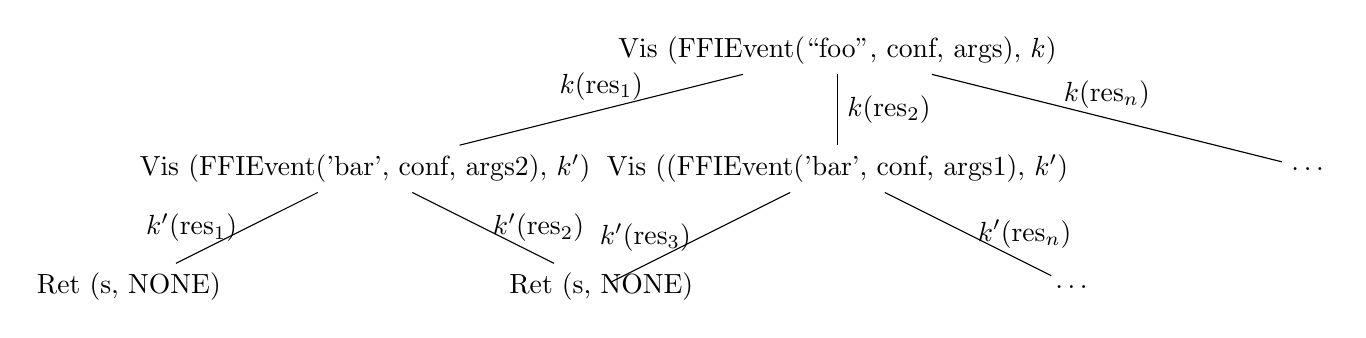
\begin{tikzpicture}[sibling distance=6cm]
      \node{Vis (FFIEvent(``foo'', conf, args), $k$)}
      child {node{Vis (FFIEvent('bar', conf, args2), $k'$)} child {node{Ret (s, NONE)} edge from parent node[left] {$k'(\text{res}_{1})$}} child {node{Ret (s, NONE)} edge from parent node[right] {$k'(\text{res}_{2})$}} edge from parent node[above] {$k(\text{res}_{1})$}}
      child {node {Vis ((FFIEvent('bar', conf, args1), $k'$)} child {node{} edge from parent node[left] {$k'(\text{res}_{3})$}} child {node{$\dots$} edge from parent node[right] {$k'(\text{res}_{n})$}} edge from parent node[right] {$k(\text{res}_{2})$}}
      child {node {$\dots$} edge from parent node[above] {$k(\text{res}_{n})$}};
    \end{tikzpicture}
  \end{adjustwidth}
    \caption{Program 1 interaction tree}
  \label{fig:prog1_tree}
\end{figure}

\section{Observational semantics}
\label{sec:obs_sem}

The observational semantics of a program is a denotation from state to ITree. The essential difference from the statement semantics is that state has been removed in the leaves (Ret terms) of the ITree.

The observational semantics is determined by the function
\begin{equation}
  \label{eq:3}
  \sem{\cdot} : \Sigma \to \text{ITree}\ \text{ExtEvent}\ \text{behaviour}.
\end{equation}

Note also that we have eschewed use of the option type as from an observational perspective the semantics are a total function onto the behaviour type.

\subsection{Definition of observational semantics}
\label{sec:defin-observ-semant}

We define $\sem{\cdot}$ as follows.

\begin{figure}[H]
  \begin{adjustwidth}{-4cm}{0pt}
  \begin{align*}
    \sem{\text{Call tail}\ n\ a_{i}} = \lambda s.\ \sem{\text{Call tail}\ n\ a_{i}}_{p} \star \lambda r.\ & \textbf{if}\ r = (s, \text{Final\_FFI}\ v)\ \lor\ r = (s, \text{Return}\ v)\ \textbf{then}\ \text{Ret}(\text{Terminate}\ v\ s.\text{ffi}.\text{io\_events})\ \\ & \textbf{else if}\ r = (s, \text{SOME Exception}\ i\ e)\ \lor\ r = (s, \text{SOME Error})\ \textbf{then}\ \text{Ret}(\text{Fail})\ \textbf{else}\ \text{Div}
  \end{align*}
  \end{adjustwidth}
  \caption{Definition of observational semantics.}
  \label{fig:sem_obs}
\end{figure}

At present, the observational semantics is defined only for tail calls to local functions. This is similar in nature to the existing observational semantics but somewhat less restrictive. The semantics can be expanded more easily from this position as the use of ITrees in Pancake semantics matures.

\end{document}
